\chapter{Workflow and Customer Journey for Coffee Chain ERP System}

This chapter details how administrators configure the system and how customers experience transactions at outlets. The workflows highlight the sequence of operations, responsibilities, and ERP automation.

\section*{System Entities}
\begin{itemize}
    \item \texttt{coffee.outlet} – Coffee Outlet details.  
    \item \texttt{res.partner} – Outlet Owner or Sale Customer.  
    \item \texttt{coffee.menu.item} – Menu Items with categories.  
    \item \texttt{sale.order} – Customer Orders linked to outlets.  
    \item \texttt{crm.lead} – Optional CRM Leads for marketing.  
\end{itemize}

\section*{Administrator Workflow}
Administrators configure the backbone of the ERP:
\begin{enumerate}
    \item Create outlet profiles, assign managers, and set operational details.  
    \item Populate the Menu Master with drinks, snacks, and pricing.  
    \item Register Sale Customers in the system for traceable transactions.  
    \item Optionally link CRM leads for customer engagement tracking.  
\end{enumerate}

\begin{figure}[H]
    \centering
    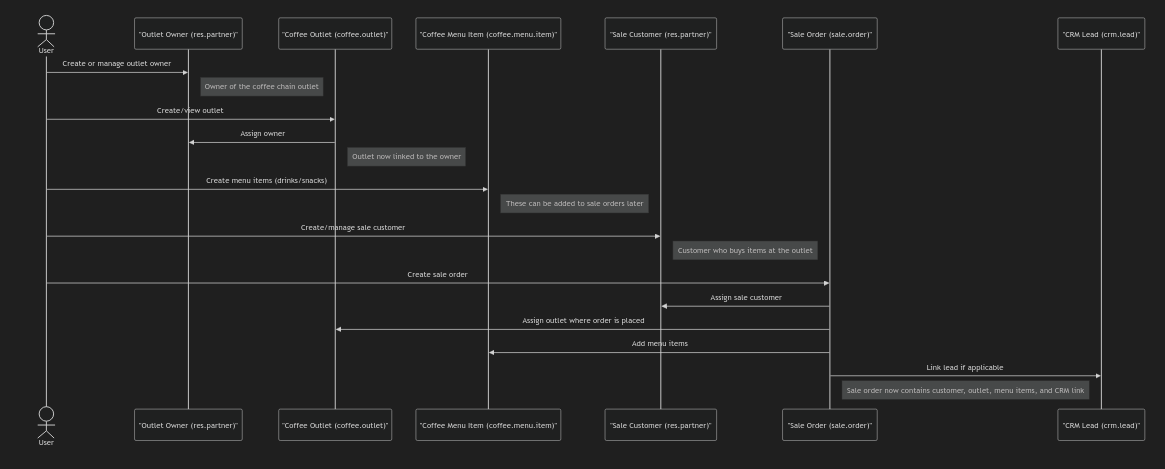
\includegraphics[width=0.85\textwidth]{diagrams/sequence.png}
    \caption{Administrator Workflow Sequence Diagram}
\end{figure}

\textbf{Why it matters:} Proper configuration ensures outlets are standardized, sales are captured accurately, and data flows without disruption.

\section*{Customer Journey at the Outlet}
The ERP supports staff during customer interactions:
\begin{enumerate}
    \item A customer places an order at the outlet counter.  
    \item Staff select the outlet profile and add the ordered menu items.  
    \item The system links the order to outlet and customer records.  
    \item The customer completes payment, and the system issues a receipt.  
    \item The transaction is saved in the database, updating reports and CRM.  
\end{enumerate}

\begin{figure}[H]
    \centering
    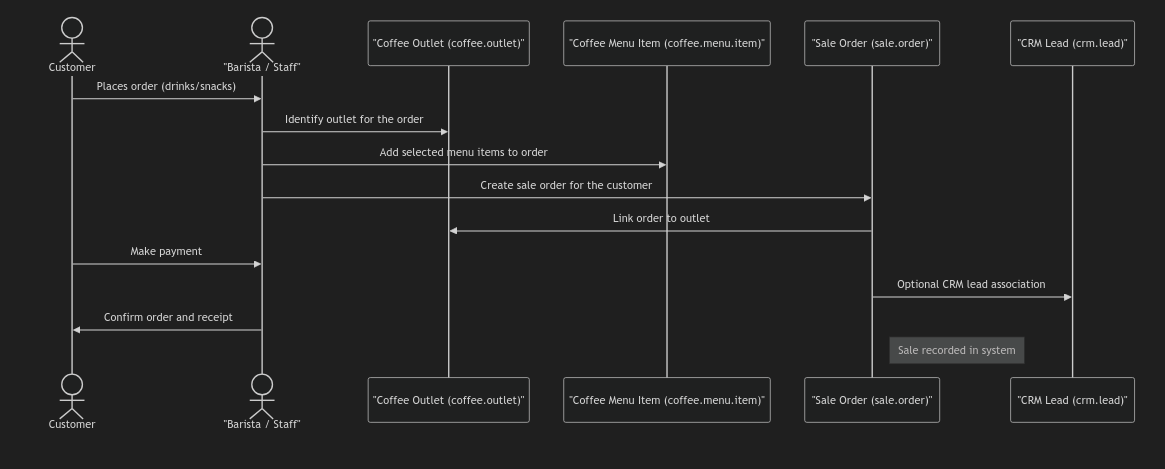
\includegraphics[width=0.85\textwidth]{diagrams/customer_journey.png}
    \caption{Customer Journey Sequence Diagram}
\end{figure}

\textbf{Why it matters:} The customer journey demonstrates how ERP integrates operations — ensuring real-time accuracy from the moment of order to final reporting.

\section*{Insights}
\begin{itemize}
    \item Administrators create the foundation; customers generate daily data.  
    \item ERP workflows ensure traceability of every transaction.  
    \item The system links customer experiences directly with business reporting.  
\end{itemize}
